
\chapter{Herramientas}

Las herramientas que necesitamos para armar una placa robotica np07 son faciles de conseguir y muy comunes para cualquier hobbista de la electronica.

\section{Soldador}

Un soldador eléctrico o de estaño, también conocido como cautín, es una herramienta eléctrica usada para soldar.
Funciona convirtiendo la energía eléctrica en calor, que a su vez provoca la fusión del material utilizado en la soldadura, como por ejemplo el estaño.

\begin{figure}[h]
	\centering
	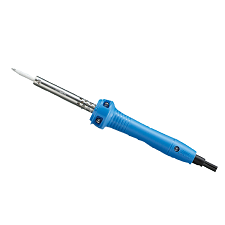
\includegraphics[width=0.5\linewidth]{herramientas/soldador}
	\caption{Soldador}
	\label{fig:soldador}
\end{figure}

\newpage

\section{Estaño}

El estaño que se utiliza en electrónica tiene alma de resina con el fin de facilitar la soldadura. 
Para garantizar una buena soldadura es necesario que tanto el estaño como el elemento a soldar alcancen una temperatura determinada, si esta temperatura no se alcanza se produce el fenómeno denominado soldadura fría. La temperatura de fusión depende de la aleación utilizada, cuyo componente principal es el estaño y suele estar comprendida entre unos 200 a 400 grados celsius.
En realidad, el término “estaño” se emplea de forma impropia porque no se trata de estaño sólo, sino de una aleación de este metal con plomo, generalmente con una proporción respectiva del 60 y del 40 por ciento, que resulta ser la más indicada para las soldaduras en Electrónica. 
Para realizar una buena soldadura, además del soldador y de la aleación descrita, se necesita una sustancia adicional, llamada pasta de soldar, cuya misión es la de facilitar la distribución uniforme del estaño sobre las super?cies a unir y evitando, al mismo tiempo, la oxidación producida por la temperatura demasiado elevada del soldador.
La composición de esta pasta es a base de colofonia (normalmente llamada “resina”) y que en el caso del estaño que utilizaremos, está contenida dentro de las cavidades del hilo, en una proporción del 2 a 2.5 por ciento.

\begin{figure}[h]
	\centering
	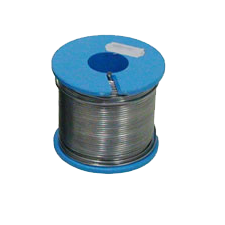
\includegraphics[width=0.5\linewidth]{herramientas/estanio}
	\caption{Estaño}
	\label{fig:estanio}
\end{figure}

\newpage

\section{Pinza}

Un pequeño alicate, para poder cortar el excedente de material (estaño, alambres de las resistensias por ejmplo).

\begin{figure}[h]
	\centering
	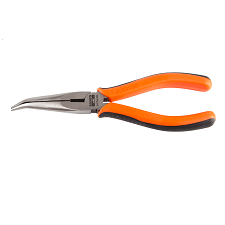
\includegraphics[width=0.5\linewidth]{herramientas/pinza}
	\caption{Alicate para Electronica}
	\label{fig:pinza}
\end{figure}

\newpage

\section{Destornillador}

Nos sirve para ajustar las borneras y para hacer palanca para sacar un integrado que hayamos puesto en un zocalo.

\begin{figure}[h]
	\centering
	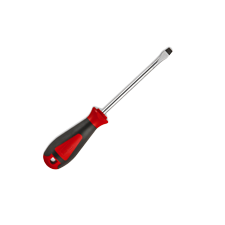
\includegraphics[width=0.5\linewidth]{herramientas/destornillador}
	\caption{Destornillador Plano Pequeño}
	\label{fig:destornillador}
\end{figure}

\newpage

\section{Desoldador de Estaño}

El desoldador de estaño, nos permite sacar el estaño que hayamos puesto de mas o para remplazar algun componente efectuoso de la placa robotica np07

\begin{figure}[h]
	\centering
	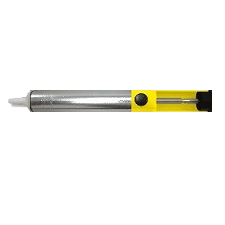
\includegraphics[width=0.5\linewidth]{herramientas/desoldador}
	\caption{Desoldador de Estaño}
	\label{fig:desoldador}
\end{figure}

